\documentclass[11pt,a4paper]{report}
\usepackage[utf8]{inputenc}
\usepackage[french]{babel}
\usepackage[T1]{fontenc}
\usepackage{amsmath}
\usepackage{amsfonts}
\usepackage{amssymb}
\usepackage{xcolor}

\usepackage{geometry}
\geometry{hmargin=2.5cm,vmargin=1.5cm}
\usepackage{wasysym}
\usepackage{graphicx}

\author{Mathieu Sarrat}
\title{LP19 - Diffraction de Fraunhofer}

\makeatletter
\renewcommand{\thesection}{\@arabic\c@section}
\makeatother


\begin{document}
\maketitle

\section*{Introduction}

La diffraction est définie par Sommerfeld comme toute déviation des rayons lumineux par rapport à leur trajet rectiligne que l'on ne peut pas expliquer par la réflexion ou par la réfraction. Le premier exposé et la première description de ce phénomène a été réalisé par Grimaldi [Diapo, scan Goodmann].\\

Selon les lois de l'optique géométrique, on s'attend à ce que l'ombre portée ait des bords nets, que le passage de la lumière à l'ombre soit brutal. Or, ce n'est pas ce que Grimaldi a observé : la transition entre ombre et lumière est progressive. On peut faire une expérience similaire, en utilisant un laser comme source lumineuse [Manip : laser rouge + fente réglable] : on voit une alternance de franges brillantes et sombres s'étendant assez loin dans l'ombre géométrique.\\

L'optique géométrique ne peut pas expliquer ce phénomène, ce qui souligne la nécessité d'une théorie ondulatoire pour décrire la lumière. Le premier a proposer un modèle ondulatoire de la lumière est Christiaan Huygens, mathématicien et physicien hollandais contemporain de Newton, partisan d'un modèle corpusculaire. Selon Huygens, tout point atteint par une onde lumineuse se comporte comme une source ponctuelle d'ondes sphériques. Fresnel, en 1818, combine le principe de Huygens à la notion d'interférences proposée par Young et parvient à calculer avec une excellente précision la répartition spatiale de l'éclairement dans les figures de diffraction. Ce sont Kirchhoff, puis Rayleigh et Sommerfeld qui mathématisent de façon rigoureuse les idées de Fresnel et Huygens (résolution d'une équation d'onde avec conditions de bord appropriées). Ces théories reposent sur une grosse approximation : celle du caractère scalaire de la lumière, ce qui revient à supposer que les composantes du champ électromagnétique constitutif de la lumière se comportement de la même façon et indépendamment les unes des autres. On néglige alors tout couplage entre ces composantes.\\ 

L'expérience montre cependant que la théorie scalaire est suffisante tant que les champs diffractés sont observés suffisamment loin de l'objet diffractant et que la taille caractéristique de celui-ci est grande devant la longueur d'onde typique de la lumière diffractée. Nous nous limiterons à cette théorie scalaire au cours de cette leçon.

\newpage
\section{Théorie scalaire de la diffraction}

\subsection{Principe d'Huygens-Fresnel}

La lumière se propage de proche en proche. Chaque élément de surface $d^2S$ atteint par elle se comporte comme une source secondaire qui émet une ondelette sphérique d'amplitude proportionnelle à l'amplitude incidente. L'amplitude en un point M est la somme de toutes les amplitudes des ondelettes issues des différentes sources secondaires.\\

Soit un point M où se trouve l'observateur et P un point courant de la surface $\Sigma$ d'élément $d^2S$.
\begin{equation}
	\Psi(M) = \iint_\Sigma d^2S\; \alpha\;  \Psi_i(P) \frac{\displaystyle{e^{ikPM}}}{PM}
\end{equation}

La théorie développée par Kirchhoff permet de donner une expression au coefficient $\alpha$,
\begin{equation}
	\alpha = -\frac{i}{\lambda}Q
\end{equation}
où $Q$ désigne le facteur d'obliquité.\\

En fait, ce principe et cette expression découlent de la linéarité des équations de Maxwell, la lumière étant une onde électromagnétique.

\subsection{Diffraction à distance finie}

On éclaire un objet diffractant $\mathcal{D}$ avec une onde plane : les rayons lumineux sont parallèles (le rayonnement laser est une bonne approximation) et arrivent avec un angle d'incidence nul sur l'objet diffractant.\\

\begin{figure}[h!]
\begin{center}
	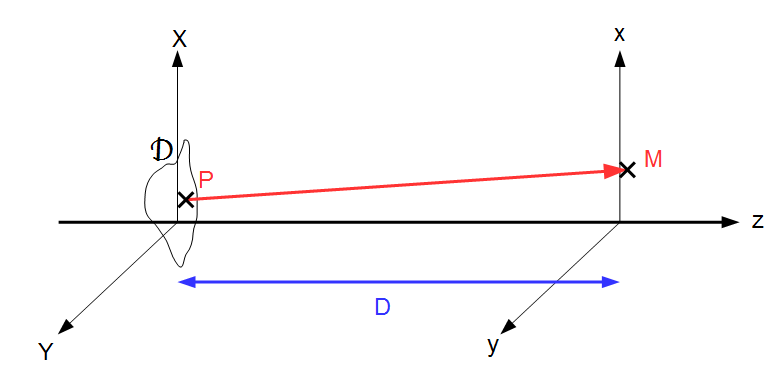
\includegraphics[scale = 0.8]{diffraction_gen.png}
	\label{fig:schema_gen}
\end{center}
\end{figure}

Définissons d'abord la transmittance de l'objet diffractant
\begin{equation}
	\tau(P) = \tau(X,Y) = \frac{\Psi(P^+)}{\Psi(P^-)} = \frac{\Psi(P^+)}{\Psi(0)}
\end{equation}
où $\Psi(P^+)$ désigne l'amplitude de l'onde au voisinage de P, juste après son passage par l'objet diffractant $\mathcal{D}$, et $\Psi(P^-)$ l'amplitude juste avant.

La transmittance est, dans le cas général, un nombre complexe. Dans le cas d'un simple trou, elle vaut 1 dans le trou et 0 en dehors : l'intégrale se réduit à l'ouverture $\mathcal{D}$.\\

De manière générale, on peut écrire :
\begin{equation}
	PM = \sqrt{\bold{PM}\cdot\bold{PM}} = D \sqrt{1 + \frac{(x-X)^2}{D^2} + \frac{(y-Y)^2}{D^2}}.\\
\end{equation}

Formulons des hypothèses :
\begin{itemize}
	\item la taille caractéristique de l'ouverture est petite devant la distance $D$ entre l'objet diffractant et l'observateur;
	\item de même, on limite l'observation à une région de taille caractéristique petite devant $D$.\\
\end{itemize}

Sous ces conditions, le facteur d'obliquité $Q$ tend vers 1 et on peut sortir le coefficient $\alpha$ (autrement source de complexité mathématique) de l'intégrale. En outre, on peut faire un développement limité de $k PM$ dans l'exponentielle :
\begin{equation}
	k PM \simeq \frac{2\pi}{\lambda} D \left(1 + \frac{(x-X)^2}{2D^2} + \frac{(y-Y)^2}{2D^2}\right) 
	=  \frac{2\pi}{\lambda} \left(D + \frac{(x-X)^2}{2D} + \frac{(y-Y)^2}{2D}\right)
\end{equation}
en se limitant à l'ordre deux du développement.\\

En toute rigueur, on devrait faire un développement à l'ordre deux dans le terme de décroissance sphérique, en $1/PM$. Cela n'est cependant pas nécessaire pour calculer avec précision la répartition spatiale de l'éclairement au niveau du plan d'observation. Ce terme de décroissance est un terme d'amplitude : il va jouer essentiellement sur la valeur absolue de l'éclairement, mais pas sur sa structure spatiale, qui sera déterminée par la terme de phase, contenu dans l'exponentielle. C'est sur ce dernier terme que la précision est nécessaire pour faire apparaître le phénomène de diffraction. Pour ces raisons et pour simplifier les calculs, on fait donc un développement à l'ordre zéro :
\begin{equation}
	\frac{1}{PM} \simeq \frac{1}{D}.
\end{equation}

L'ensemble de ces approximations correspond à un régime que l'on appelle \textbf{diffraction de Fresnel}, ou encore diffraction à distance finie. Dans ce régime, l'intégrale de diffraction s'écrit :
\begin{equation}
	\Psi(M) =  \alpha \Psi_0 \iint_\mathcal{D} dXdY\; \tau(X,Y) \displaystyle{\frac{e^{ikD}}{D}}\displaystyle{\text{exp}\left(i\frac{k}{2D}\left( (x-X)^2 + (y-Y)^2 \right)\right)}\\
\end{equation}

Vérifions numériquement si ces hypothèses sont facilement réalisables sur un banc d'optique 
($\lambda \simeq 1 \mu m$, $R = \sqrt{X^2 + Y^2} \simeq 1\;\text{mm}$, $D \simeq 1\;\text{m}$) :\\
\begin{itemize}
	\item terme d'ordre 2 :
	\begin{equation}
		\frac{2\pi}{\lambda} \frac{R^2}{D} \simeq 2\pi\\
	\end{equation}
	
	\item terme d'ordre 4 :
	\begin{equation}
		\frac{2\pi}{\lambda} \frac{R^4}{D^3} \simeq 2\pi 10^{-6}.
	\end{equation}
\end{itemize}

Le terme d'ordre 4 est bien négligeable, et il l'est d'autant plus que $R$ est faible : on obtient donc très facilement de la diffraction sur un banc d'optique en utilisant de petits objets, comme des fentes.

\newpage
\section{Diffraction à l'infini}

Le calcul de l'intégrale précédente est délicat, du fait de la présence du terme en $X^2 + Y^2$. Le recours aux fonctions spéciales est nécessaire. Si on se place suffisamment loin de l'objet diffractant, le terme quadratique tend vers 0. Ces conditions plus restrictives, mais pour lesquelles il est possible de calculer analytiquement la forme de la figure de diffraction, correspondent au régime de Fraunhofer, aussi appelé diffraction à l'infini.
 
\subsection{Approximation de Fraunhofer}

\subsubsection{Régime de Fraunhofer approché :}
L'approximation de Fraunhofer consiste à négliger le terme quadratique en $X^2 + Y^2$. Ce terme est de l'ordre de
\begin{equation}
	\frac{k R^2}{2 D} = \frac{\pi R^2}{\lambda D},
\end{equation}
où $R$ est la taille caractéristique de l'objet diffractant \footnote{On soulignera le fait qu'un bord d'écran n'a pas de taille caractéristique $R$, et que par conséquent la figure de diffraction qu'il génère ne peut être étudiée qu'en régime de Fresnel.}. Le terme quadratique est négligeable si
\begin{equation}
	\frac{R^2}{\lambda D} \ll 1 \leftrightarrow R^2 \ll \lambda D \quad\text{ou}\quad D \gg \frac{R^2}{\lambda}.
\end{equation}

On parle de régime de Fraunhofer approché lorsque cette inégalité est bien vérifiée par le montage de diffraction étudié :
\begin{itemize}
	\item si $R \sim 1 mm$ et $\lambda \sim 1 \mu m$, le régime de Fraunhofer approché est atteint pour $D \gg 1$, ce qui n'est jamais réalisé sur une paillasse,
	\item si $R \sim 0.1 mm$ et $\lambda \sim 1 \mu m$, le régime de Fraunhofer approché est atteint pour $D \gg 1 cm$, ce qui est faisable en pratique avec un banc d'optique.
\end{itemize}
Dans le cas où cette inégalité est vérifiée, on néglige le terme quadratique dans l'intégrale précédente, qui devient :
\begin{equation}
	\Psi(M) \simeq  \alpha \Psi_0 \displaystyle{\frac{e^{ikD}}{D}}\displaystyle{\text{exp}\left(i\frac{k}{2D}(x^2 + y^2) \right)} \iint_\mathcal{D} dXdY\; \tau(X,Y) \displaystyle{\text{exp}\left(-i 2\pi \frac{xX + yY}{\lambda D}\right)}\\
\end{equation}

\subsubsection{Régime de Fraunhofer strict :}

Pour réaliser strictement la limite de Fraunhofer, il faudrait se placer à une distance infinie par rapport à l'objet diffractant. Une façon pratique de réaliser cette limite est de positionner l'écran d'observation dans le plan focal image d'une lentille convergente de longueur focale $f$ : on ramène la figure de diffraction à l'infini dans le plan focal de la lentille.\\

Reprenons l'intégrale
\begin{equation}
	\Psi(M) \propto \Psi_0 \iint_\mathcal{D} dXdY \tau(X,Y) \frac{\displaystyle{e^{ikPM}}}{D},
\end{equation}
dans laquelle on fait passer $1/D$ dans la constante multiplicative devant l'intégrale (on omettra ce $D$ à l'avenir).\\

La quantité $kPM$ peut s'écrire
\begin{equation}
	k PM = k_0 L(PM),
\end{equation}
où $L(PM)$ correspond au chemin optique parcouru par un rayon émergeant du diaphragme avec un angle $\theta$. \'Ecrivons
\begin{equation}
	L(PM) = L(OM) + L(PM) - L(OM) = L(OM) + \delta,
\end{equation}
où $\delta$ est la différence de chemin optique entre deux rayons émergeant avec le même angle $\theta$, celui passant par P et celui passant par O.\\

Pour simplifier le calcul de $\delta$, on se limite à une seule dimension mais on pourra généraliser le résultat à deux dimensions. Faisons apparaître $H$, de sorte que $L(OM) = L(HM)$. Ainsi,
\begin{equation}
	\delta = L(PH) = - \text{sin}\theta\;OP = - \text{sin}\theta\;X.
\end{equation}
Le signe $-$ est nécessaire : $X < 0$ sur le schéma, alors que $PH$ et $\text{sin}\theta$ sont positifs.\\

La lentille est utilisée dans l'approximation de Gauss : les rayons passent au voisinage de l'axe optique et sont faiblement inclinés par rapport à celui-ci. Ces conditions sont compatibles avec celles supposées pour obtenir le régime de Fraunhofer. Ainsi : 
\begin{equation}
	\text{sin}\theta \simeq \text{tan}\theta \simeq \frac{x}{f},
\end{equation}
d'où
\begin{equation}
	PH = - \frac{xX}{f}.
\end{equation}

En généralisant à 2D, on obtient
\begin{equation}
	\delta = - \frac{xX + yY}{f}.
\end{equation}
Comme les rayons arrivent en phase sur le diaphragme (faisceau incident parallèle à l'axe optique) il n'y a pas de différence de chemin optique supplémentaire à prendre en compte du fait du parcours de la lumière avant qu'elle n'atteigne le diaphragme.

L'intégrale de diffraction s'écrit alors
\begin{equation}
	\Psi(M) \propto \Psi_0 \iint_\mathcal{D} dXdY \tau(X,Y) \text{exp}\left( - i 2\pi \frac{xX + yY}{\lambda f}\right),
\end{equation}
dans laquelle il n'existe pas de terme quadratique en $X^2 + Y^2$, celui-ci ayant été éliminé par l'action de la lentille convergente. On réalise donc exactement le régime de Fraunhofer.\\

On définit maintenant deux quantités 
\begin{equation}
	u \equiv \frac{x}{\lambda f} \quad\text{et}\quad v \equiv \frac{y}{\lambda f},
\end{equation}
homogènes à l'inverse d'une longueur. On les appelle \textbf{fréquences spatiales}. En effet, on reconnaît dans l'intégrale de diffraction en régime de Fraunhofer la transformée de Fourier de la transmittance $\tau$ :
\begin{equation}
	\Psi(M) \propto \Psi_0 \iint_\mathcal{D} dXdY \tau(X,Y) \text{exp}\left( - i 2\pi \left( uX + vY \right) \right),
\end{equation}
que l'on réécrira comme une fonction des fréquences spatiales
\begin{equation}
	\Psi(u,v) \propto \Psi_0 \text{TF}\left[\tau \right].
\end{equation}

\newpage
\subsection{Quelques figures de diffraction}
 
\subsubsection{Cas d'une ouverture rectangulaire}

Soit une ouverture rectangulaire, de dimensions $a$ (horizontale, selon $X$) et $b$ (verticale, selon $Y$). La transmittance s'écrit
\begin{equation}
	\tau(X,Y) = \text{rect}\left(\frac{X}{a}\right)\text{rect}\left(\frac{Y}{b}\right),
\end{equation}
de sorte que $\tau$ vaut 1 pour $|X| < a/2$ et $|Y| < b/2$ et 0 autrement.\\

Ainsi,
\begin{equation}
	\Psi(u,v) \propto \Psi_0 \int_{-a/2}^{a/2}dX\; \text{exp}(-i2\pi uX)   \int_{-b/2}^{b/2}dY\; \text{exp}(-i2\pi vY).
\end{equation}

On en déduit l'éclairement dans le plan $(x,y)$ :
\begin{equation}
	\mathcal{E}(u,v) = |\Psi(u,v)|^2 \propto \mathcal{E}_0 \text{sinc}^2(\pi u a) \text{sinc}^2(\pi v b)
\end{equation}
où $\mathcal{E}_0$ désigne l'éclairement au centre de la tache principale et où $\text{sinc}(X) = \text{sin}(X)/X$ est la fonction sinus cardinal.\\

\textcolor{red}{Photo de la figure de diffraction}.

Cette fonction vaut 1 pour $u$ = 0, ce qui correspond au maxima d'éclairement de la tache centrale. La fonction sinus cardinal s'annule quasi-périodiquement, puisque pour $X \neq 0$,
\begin{equation}
	\text{sinc}(X) = 0 \quad\text{ssi}\quad \text{sin}(X) = 0,
\end{equation}
c'est à dire si 
\begin{equation}
	X = n\pi, 
\end{equation}
où $n$ désigne un entier relatif, différent de 0. Il y a donc un espacement régulier des "zéros" de l'éclairement.\\

Intéressons nous en l'occurrence à la diffraction selon la direction $x$. On obtient un "zéro de l'éclairement" selon $x$ si
\begin{equation}
	u a = n, \qquad\text{donc pour}\qquad u_n = \frac{n}{a}, \quad\text{avec}\quad n \neq 0,\; \text{entier relatif}.
\end{equation}
Les zéros sont donc d'autant plus proches que $a$, la dimension caractéristique de l'objet diffractant selon $X$, est grande. Le même raisonnement s'applique à la direction $Y$. C'est le phénomène d'\textbf{inversion des échelles} : plus la taille de l'objet diffractant est petite, plus les taches de diffraction seront larges.

\subsubsection{Cas d'une fente rectangulaire}

C'est par ce raisonnement que l'on peut prédire la forme de la tache de diffraction générée par une fente, telle que $a \ll b$ : il n'a presque plus plus de lumière en dehors de $v = 0$. L'éclairement s'écrit :
\begin{equation}
	\mathcal{E}(u,v) \simeq \mathcal{E}(u) \propto \mathcal{E}_0\;\text{sinc}^2(\pi u a).
\end{equation}

\textcolor{red}{Tracer la figure de diffraction au tableau.} 

Soit $\mathcal{E}_1$ l'éclairement au niveau du premier maximum secondaire. Le rapport
\begin{equation}
	\frac{\mathcal{E}_1}{\mathcal{E}_0} \simeq 4\%.
\end{equation}

On se propose de vérifier quantitativement l'espacement régulier des zéros de la figure de diffraction. \textcolor{red}{Expérience quantitative : montage en Fraunhofer approché, mesures réalisées en préparation, expliquer seulement le principe. On pointe les zéros de l'éclairement, que l'on numérote de $-n$ à $+n$. On trace la position des zéros en fonction de $n$. On trace les résidus dont on étudie la répartition, on en déduit un ordre de grandeur de l'incertitude sur le pointé, on conclut. On mesure ensuite une valeur de $i = \lambda D/a$ que l'on compare à la valeur obtenue connaissant $a$ (fente calibrée), $\lambda$ (laser vert, incertitude négligée), $D$ (mesurée). Calcul des incertitudes, montrer qu'elles se recouvrent.}

\subsection{Propriétés des figures de diffraction}
\textcolor{red}{Partie à sauter si manque de temps, compte tenu de l'expérience précédente...}

\subsubsection{Translation de $\mathcal{D}$ dans un plan perpendiculaire à l'axe optique}

La translation de $\mathcal{D}$ dans un tel plan ne fait que multiplier l'amplitude complexe par un terme de phase, qui disparaît une fois qu'on calcule l'intensité. Illustrer expérimentalement. Calcul, si le temps le permet : remplacer $\tau(X,Y)$ par $\tau'(X,Y) = \tau(X-X_0,Y-Y_0)$

\subsubsection{Théorème de Babinet}

On l'appelle aussi théorème des écrans complémentaires : les figures de diffraction générées par un objet de transmittance $\tau_c$, 
\begin{equation}
	\tau_c(X,Y) = 1 - \tau(X,Y)
\end{equation}
complémentaire de celle d'un objet de transmittance $\tau$, et par l'objet de transmittance $\tau$ sont identiques à l'exception du centre. Illustrer expérimentalement en remplaçant la fente par un trait de même largeur.

\section{Rôle de la diffraction dans la formation des images}

Nous allons voir que le phénomène de diffraction joue un rôle important dans la formation des images.

\subsection{Rotation de l'éclairage}

Jusqu'à présent dans notre modèle, la fente était éclairée par un faisceau de rayons parallèles aligné le long de l'axe optique. On fait maintenant tourner la source, de sorte que le faisceau incident forme un angle $\theta_0$ avec l'axe optique. Deux rayons émis avec le même angle $\theta$ depuis $\mathcal{D}$ (et convergeant donc au point M sur l'écran placé dans le plan focal image de la lentille) ne sont plus en phase au moment où ils arrivent sur le diaphragme. Ainsi, l'amplitude complexe correspondant aux rayons émis depuis $\mathcal{D}$ selon la direction fixée par $\theta$ s'écrit
\begin{equation}
	\Psi(P^+) = \tau(X,Y)\Psi_0 \;\text{exp}\left(i\Phi(P)\right),
\end{equation}
où $\Phi(P)$, la phase de l'onde incidente, dépend désormais du point d'impact sur $\mathcal{D}$. On choisit comme référence $\Phi(O) = 0$, pour être cohérent avec le choix fait pour calculer la différence de marche entre deux rayons parallèles après $\mathcal{D}$.\\

Pour simplifier le calcul, on se replace dans un cas 1D, mais on pourra généraliser au cas 2D $(X,Y)$. D'après le schéma, dans l'air,
\begin{equation}
	\Phi(P) = \Phi(O) - k KO = - \frac{2\pi}{\lambda}KO,
\end{equation}
et
\begin{equation}
	KO = - X \text{sin}(\theta_0), \quad\text{d'où}\quad \Phi(P) = \frac{2\pi}{\lambda} X \text{sin}(\theta_0).
\end{equation}
Or, les angles étant petits,
\begin{equation}
	\text{sin}(\theta_0) \simeq \text{tan}\theta_0 = \frac{x_0}{f},
\end{equation}
d'où
\begin{equation}
	\Psi(P^+) = \tau(X)\Psi_0 \text{exp}\left(i2\pi\frac{x_0 X}{\lambda f}\right).\\
\end{equation}

L'amplitude de l'onde reçue au point M s'écrit
\begin{equation}
	\Psi(x) \propto \Psi_0 \int_\mathcal{D} dX\; \tau(X) \displaystyle{e^{-i2\pi\frac{(x-x_0)X}{\lambda f}}}.
\end{equation}
et
\begin{equation}
	\Psi(x,y) \propto \Psi_0 \int_\mathcal{D} dXdY\; \tau(X,Y) \displaystyle{e^{-i2\pi\frac{(x-x_0)X + (y-y_0)Y}{\lambda f}}}.
\end{equation}
dans le cas à deux dimensions.

Le changement de variable
\begin{equation}
	u \equiv \frac{x - x_0}{\lambda f} \quad\text{et}\quad v \equiv \frac{y - y_0}{\lambda f}
\end{equation}
nous montre qu'on obtient exactement la même figure de diffraction dans l'espace $(u,v)$ que dans le cas où la source est positionnée sur l'axe optique. Dans l'espace $(x,y)$, la figure de diffraction est simplement translatée autour du point $(x_0,y_0)$, point qui est par ailleurs l'image de la source par la lentille convergente.\\

Nous venons de démontrer que \textbf{la figure de diffraction entoure l'image géométrique}. En déplaçant l'objet, on déplace son image, et la figure de diffraction suit le mouvement.

\subsection{Critère de Rayleigh}

Nous venons de voir que s'il y avait diffraction de la lumière sur son trajet entre un point objet et son image conjuguée, la figure de diffraction se formait autour du point image, devenu en quelque sorte une tache image. Cette situation, au premier abord, peut paraître assez superficielle. Après tout, y a-t-il toujours diffraction lorsqu'on forme une image ?\\

Nous avons vu qu'un bord d'écran était suffisant pour provoquer le phénomène de diffraction. Les systèmes optiques couramment utilisés, par exemple des lentilles, possèdent des montures qui limitent transversalement le passage de la lumière : cela suffit à créer une figure de diffraction. Dans le cas où la monture est circulaire, la figure de diffraction est une tache d'Airy \textcolor{red}{[Diapo]}. La position du premier zéro de l'éclairement est donnée par (coordonnées cylindriques) :
\begin{equation}
	r_1 = 1.22 \frac{\lambda f}{2R},
\end{equation}
où $R$ est le rayon du trou circulaire diffractant (par exemple, le rayon de la monture d'une lentille convergente).

Ainsi, tout point objet forme une tache de diffraction sur un écran après passage par un instrument d'optique, d'autant plus petite que l'instrument d'optique a une taille importante. Cela implique l'existence d'une limite de résolution pour tout instrument d'optique, cette limite étant causée par la diffraction. Au-delà de cette limite, il est donc impossible de distinguer deux points objets trop proches l'un de l'autre.\\ 

Le critère de Rayleigh permet de préciser cette limite : ce critère est atteint lorsqu'on ne peut plus distinguer deux objets du fait de la diffraction : les deux taches de diffraction n'en font plus qu'une. \textcolor{red}{On peut éventuellement faire une manip : bifente, fente réglable, lentille convergente, condenseur, lampe QI et caméra CCD.}

\newpage
\section{Conclusion}
\begin{itemize}
	\item récapitulatif.
	\item ouverture sur la diffraction par des structures périodiques.
	\item ouverture sur l'optique de Fourier et le traitement des images en utilisant la notion de fréquence spatiale.
\end{itemize}

\end{document}